\chapter{Statistische thermodynamica: toestandssommen}\label{ch:b3:partition-functions}

Op het graf van Ludwig Boltzmann in Wenen staat één enkele regel, $S = k\log W$: de
entropie van een systeem telt de manieren waarop zijn moleculen zijn
energie kunnen verdelen. De thermodynamica zoals de delen van jaar~1 en
jaar~2 haar opbouwden, heeft nooit moleculen nodig: ze verbindt gemeten
warmten, entropieën en evenwichtsconstanten met elkaar. De statistische
thermodynamica berekent ze uit de moleculen zelf. Haar centrale object is
één enkele som over de energieniveaus van één molecuul, de toestandssom;
de niveaus komen uit de spectroscopie, en de standaardentropie van
stikstof, berekend uit zijn spectrum, stemt tot op een honderdste joule per
kelvin en per mol overeen met de getabelleerde waarde. Dit hoofdstuk bouwt
de toestandssom op, splitst haar in haar translatie-, rotatie-, vibratie-
en elektronische delen, en zet haar om in inwendige energie, entropie en
gibbsenergie; \cref{ch:b3:statistical-thermo-applied} past haar toe op
warmtecapaciteiten en evenwichtsconstanten.

\begin{recall}
Het deel van jaar~2 definieerde de standaard molaire entropie, de
gibbsenergie en de chemische potentiaal, en zette entropieën in tabellen
die verkregen werden uit warmtecapaciteiten gemeten tot bij lage
temperatuur. \Cref{ch:b3:quantum-model-systems} gaf de energieniveaus van
een \omterm{def:b3:quantum-model-systems:box}{deeltje in een doos}, van de \omterm{def:b3:quantum-model-systems:oscillator}{harmonische oscillator} en van de \omterm{def:b3:quantum-model-systems:rotor}{starre
rotor}, $E_J = hcBJ(J+1)$ met \omterm{def:b3:quantum-model-systems:degenerate}{ontaardingsgraad} $2J + 1$;
\cref{ch:b3:rovibrational-spectroscopy} mat $B$ en $\tilde\nu$ voor
diatomische moleculen en vond dat in een homonucleair molecuul zoals
\ce{N2} de kernspins om de beurt rotatieniveaus ongelijk maken.
\end{recall}

\section{Microtoestanden en de boltzmannverdeling}

Beschouw $N$ identieke, onafhankelijke moleculen die niveaus met energie
$\varepsilon_0 = 0 < \varepsilon_1 < \varepsilon_2 < \dots$ kunnen bezetten, met totale energie $E$. Zeggen hoeveel
moleculen zich op elk niveau bevinden, $\{n_0, n_1, \dots\}$, beschrijft een
verdeling; zeggen welk molecuul op welk niveau zit, beschrijft veel meer.

\begin{definition}[Microtoestand, statistisch gewicht]\label{def:b3:partition-functions:microstate}
Een \emph{microtoestand}\index{microtoestand} van een systeem van moleculen
is een volledige specificatie van de toestand van elk molecuul. Het
\emph{statistisch gewicht}\index{statistisch gewicht} $W$ van een verdeling
$\{n_i\}$ van $N$ moleculen over
niet-ontaarde niveaus is het aantal microtoestanden dat haar realiseert:
\[
  W = \frac{N!}{n_0!\,n_1!\,n_2!\cdots}.
\]
\end{definition}

\begin{example}[Drie kwanta over drie oscillatoren]\label{ex:b3:partition-functions:three-quanta}
Drie oscillatoren delen drie energiekwanta. De verdeling ``één oscillator
heeft ze alle drie'' kan op $3!/(1!\,2!) = 3$ manieren gerealiseerd worden,
``één heeft er twee, een andere één'' op $3! = 6$ manieren en ``elk heeft
er één'' op één manier: tien \omterm{def:b3:partition-functions:microstate}{microtoestanden} in totaal, en de meest
gelijkmatige verdeling die de energie toch over meerdere niveaus spreidt,
is de waarschijnlijkste. Met $10^{23}$ moleculen worden de gewichten zo
scherp gepiekt dat één verdeling, samen met de verdelingen die er
verwaarloosbaar weinig van verschillen, praktisch alle \omterm{def:b3:partition-functions:microstate}{microtoestanden}
draagt.
\end{example}

\begin{remark}
Het postulaat van de statistische thermodynamica is dat alle
\omterm{def:b3:partition-functions:microstate}{microtoestanden} van een geïsoleerd systeem met een gegeven energie even
waarschijnlijk zijn. Het systeem wordt dan overweldigend vaak aangetroffen
in de verdeling met het grootste gewicht: die vinden is de taak van deze
paragraaf.
\end{remark}

Voor grote getallen geeft de benadering van Stirling $\ln x! \approx x\ln x - x$
\[
  \ln W = N\ln N - \sum_i n_i\ln n_i .
\]

\begin{definition}[Boltzmannverdeling, bezetting]\label{def:b3:partition-functions:boltzmann}
De \emph{bezetting}\index{bezetting} $n_i/N$ van een niveau is de fractie
van de moleculen die het bezetten. De
\emph{boltzmannverdeling}\index{boltzmannverdeling}
is de verdeling met het grootste gewicht van onafhankelijke moleculen in
thermisch evenwicht bij temperatuur $T$, gegeven door de stelling
hieronder.
\end{definition}

\begin{theorem}[De boltzmannverdeling]\label{thm:b3:partition-functions:boltzmann}
Voor onafhankelijke moleculen in evenwicht bij temperatuur $T$ is de
bezetting van een niveau met energie $\varepsilon_i$ en \omterm{def:b3:quantum-model-systems:degenerate}{ontaardingsgraad} $g_i$
\[
  \frac{n_i}{N} = \frac{g_i\eu^{-\varepsilon_i/kT}}{q},
  \qquad q = \sum_i g_i\eu^{-\varepsilon_i/kT},
\]
waarin $k$ de boltzmannconstante is. Twee niveaus hebben \omterm{def:b3:partition-functions:boltzmann}{bezettingen} in de
verhouding
$\frac{n_j}{n_i} = \frac{g_j}{g_i}\eu^{-(\varepsilon_j - \varepsilon_i)/kT}$.
\end{theorem}

\begin{proof}[Gedeeltelijk bewijs]
Neem eerst niet-ontaarde niveaus. Maximaliseer $\ln W$ onder de twee
voorwaarden
$\sum_in_i = N$ en $\sum_in_i\varepsilon_i = E$ met lagrangemultiplicatoren $\alpha$ en $\beta$:
voor elke $i$ is
\[
  \frac{\partial}{\partial n_i}\Bigl(\ln W + \alpha\sum_jn_j - \beta\sum_jn_j\varepsilon_j\Bigr)
  = -\ln n_i - 1 + \alpha - \beta\varepsilon_i = 0,
\]
dus $n_i = \eu^{\alpha - 1}\eu^{-\beta\varepsilon_i}$, en de eerste voorwaarde legt $\eu^{\alpha - 1}
= N/\sum_j\eu^{-\beta\varepsilon_j}$ vast. Een niveau met \omterm{def:b3:quantum-model-systems:degenerate}{ontaardingsgraad} $g_i$ bestaat uit $g_i$
verschillende toestanden met dezelfde energie, elk bezet zoals hierboven:
zijn \omterm{def:b3:partition-functions:boltzmann}{bezetting} wordt vermenigvuldigd met
$g_i$. De multiplicator $\beta$ wordt vastgelegd met één bekend geval: voor
de translatiebeweging van een ideaal gas (\cref{prop:b3:partition-functions:q-trans}
hieronder) geeft de verdeling een energie $\frac32N/\beta$, en de energie
van een ideaal gas is $\frac32NkT$; dus $\beta = 1/kT$. Dat $\beta$ dezelfde
grootheid is voor elk soort beweging, en dat het de thermodynamische
temperatuur is, wordt hier aangenomen: twee systemen in thermisch contact
delen dezelfde $\beta$, wat de bepalende eigenschap van de temperatuur is.
\end{proof}

\begin{definition}[Moleculaire toestandssom]\label{def:b3:partition-functions:partition-function}
De \emph{moleculaire toestandssom}\index{moleculaire toestandssom} van een
molecuul bij temperatuur $T$ is de som
\[
  q = \sum_{\text{niveaus}}g_i\eu^{-\varepsilon_i/kT} = \sum_{\text{toestanden}}\eu^{-\varepsilon_s/kT},
\]
met energieën gemeten vanaf het laagste niveau, zodat $q \ge 1$.
\end{definition}

De toestandssom telt de toestanden die thermisch toegankelijk zijn: bij
zeer lage temperatuur draagt alleen het laagste niveau bij en $q \to g_0$; bij zeer
hoge temperatuur draagt elke toestand ongeveer 1 bij en groeit $q$ zonder
grens. Daaruit volgt een vuistregel: niveaus die veel meer dan $kT$ boven
het laagste liggen, zijn leeg, niveaus binnen $kT$ ervan zijn bezet. Bij
\qty{298.15}{K} komt $kT$ overeen met
\qty{207.2}{cm^{-1}}, of $RT = \qty{2.479}{kJ/mol}$.

\begin{method}[Bezettingen van niveaus uit spectroscopische constanten]\label{met:b3:partition-functions:populations}
\begin{enumerate}
  \item Maak een lijst van de niveaus met hun energieën (uit de constanten,
        bijvoorbeeld $hcBJ(J+1)$) en ontaardingsgraden ($2J + 1$).
  \item Druk elke energie uit in eenheden van $kT$; deel bij
        \qty{298.15}{K} een golfgetal door \qty{207.2}{cm^{-1}}.
  \item Vorm de termen $g_i\eu^{-\varepsilon_i/kT}$, tel ze op om $q$ te krijgen, en deel.
        Stop de som wanneer de termen verwaarloosbaar worden.
  \item Controle: de \omterm{def:b3:partition-functions:boltzmann}{bezettingen} tellen op tot 1; de verhouding van twee
        ervan is
        $\frac{g_j}{g_i}\eu^{-(\varepsilon_j-\varepsilon_i)/kT}$.
\end{enumerate}
\end{method}

\begin{example}[De rotatieniveaus van waterstofchloride]\label{ex:b3:partition-functions:hcl}
% ledger: diat:HCl.Be, diat:HCl.ae
Voor \ce{H^{35}Cl} is $B_0 = B_e - \alpha_e/2 = \qty{10.44}{cm^{-1}}$. Bij
\qty{300}{K} ligt het niveau $J$
bij $10.44\,J(J+1)$~\unit{cm^{-1}}, dus bij $0.0501\,J(J+1)$ in eenheden van $kT$. De termen
$(2J+1)\eu^{-0.0501J(J+1)}$ zijn 1, 2.71, 3.70, 3.84, 3.31, 2.45, \dots; hun som is
$q = 20.3$ en de \omterm{def:b3:partition-functions:boltzmann}{bezettingen} van $J = 0$ tot 4 zijn 0.049, 0.134, 0.182, 0.189 en
0.163: het sterkst bezette niveau is $J = 3$, niet $J = 0$, omdat de
\omterm{def:b3:quantum-model-systems:degenerate}{ontaardingsgraad}
$2J + 1$ groeit terwijl de boltzmannfactor daalt. Dit is de omhullende van
de rotatie-vibratieband van \cref{ch:b3:rovibrational-spectroscopy}.
\end{example}

\begin{omfigure}
\begin{tikzpicture}[font=\small]
  % levels J = 0-3, g = 2J+1, energies 0, 1, 3, 6 (units of 2hcB); bars = 3.5 cm x population
  % of the four levels alone at kT = 2hcB (0.422, 0.466, 0.105, 0.007) and kT = 10hcB (0.120, 0.296, 0.330, 0.254)
  \foreach \J/\e/\g/\lo/\hi in {0/0/1/1.48/0.42, 1/1/3/1.63/1.04, 2/3/5/0.37/1.16, 3/6/7/0.03/0.89}{
    \draw[thick] (0,0.55*\e) -- (2.2,0.55*\e);
    \node[anchor=east] at (0,0.55*\e) {$J = \J$};
    \node[anchor=west, font=\scriptsize] at (2.25,0.55*\e) {$g = \g$};
    \fill[omDef!70] (3.4,0.55*\e-0.11) rectangle ++(\lo,0.22);
    \fill[omThm!70] (6.4,0.55*\e-0.11) rectangle ++(\hi,0.22);
  }
  \node[anchor=south, omDef] at (4.2,3.6) {lage $T$};
  \node[anchor=south, omThm] at (7.2,3.6) {hoge $T$};
  \draw[->] (-1.4,0) -- (-1.4,3.7) node[anchor=south] {$\varepsilon$};
\end{tikzpicture}

{\small Een boltzmanntrap: de rotatieniveaus $J = 0$ tot 3 (energieën $0$,
$2$, $6$,
$12$ maal $hcB$, ontaardingsgraden $2J + 1$) en hun \omterm{def:b3:partition-functions:boltzmann}{bezettingen}, als
lengten van balken,
bij $kT = 2hcB$ en $kT = 10hcB$ (alleen de vier niveaus). Opwarmen maakt het
laagste niveau leger ten voordele van de hogere; bij beide temperaturen
tellen de balken op tot hetzelfde totaal, het aantal moleculen.}
\end{omfigure}

\section{De moleculaire toestandssom}

\begin{proposition}[Factorisatie]\label{prop:b3:partition-functions:factorisation}
Als de energie van een molecuul een som is van onafhankelijke bijdragen,
$\varepsilon = \varepsilon^{\mathrm T} + \varepsilon^{\mathrm R} + \varepsilon^{\mathrm V} + \varepsilon^{\mathrm E}$, waarbij elke toestand
een willekeurige combinatie is van een translatie-, een rotatie-, een
vibratie- en een elektronische toestand, dan is
\[
  q = q^{\mathrm T}q^{\mathrm R}q^{\mathrm V}q^{\mathrm E}.
\]
\end{proposition}

\begin{proof}
De som over alle combinaties van een exponentiële van een som is het
product van de afzonderlijke sommen: $\sum_{a,b}\eu^{-(\varepsilon_a+\varepsilon_b)/kT} = \bigl(\sum_a\eu^{-\varepsilon_a/kT}\bigr)
\bigl(\sum_b\eu^{-\varepsilon_b/kT}\bigr)$, en evenzo voor vier factoren.
\end{proof}

De scheiding is een benadering: rotatie en vibratie wisselwerken (de
constante $\alpha_e$), en de elektronische toestand bepaalt de rotatie- en
vibratieconstanten. Voor een molecuul in zijn elektronische grondtoestand
bij gewone temperaturen bedragen de fouten enkele honderdsten joule per
kelvin in een entropie. De \omterm{def:b3:partition-functions:boltzmann}{bezettingen} worden dan voor elk soort beweging
afzonderlijk berekend: de fractie moleculen in een vibratieniveau $v$
hangt niet af van hun rotatie.

\section{De vier bijdragen}

\subsection*{Translatie}

\begin{definition}[Thermische golflengte]\label{def:b3:partition-functions:thermal-wavelength}
De \emph{thermische golflengte}\index{thermische golflengte} van een
molecuul met massa $m$ bij temperatuur $T$ is
$\Lambda = \dfrac{h}{\sqrt{2\pi mkT}}$.
\end{definition}

\begin{proposition}[Translatietoestandssom]\label{prop:b3:partition-functions:q-trans}
Voor een molecuul met massa $m$ dat vrij kan bewegen in een volume $V$ is
\[
  q^{\mathrm T} = \frac{V}{\Lambda^3}.
\]
\end{proposition}

\begin{proof}
In één dimensie heeft een doos met lengte $L$ de niveaus $\varepsilon_n = h^2n^2/8mL^2$
($n = 1, 2, \dots$; de nulpuntsverschuiving verandert niets meetbaars). Ze
liggen zo dicht bij elkaar dat de som een integraal is:
\[
  q_x = \sum_{n\ge1}\eu^{-h^2n^2/8mL^2kT} \approx \int_0^\infty\eu^{-h^2n^2/8mL^2kT}\dd n
      = \frac12\sqrt{\frac{\pi\,8mL^2kT}{h^2}} = \frac{L\sqrt{2\pi mkT}}{h} = \frac{L}{\Lambda}.
\]
De drie richtingen zijn onafhankelijk: $q^{\mathrm T} = q_xq_yq_z = L^3/\Lambda^3$. De
gemiddelde energie per dimensie is $-\partial\ln q_x/\partial\beta$ met $q_x \propto \beta^{-1/2}$, dus
$1/2\beta$; drie dimensies geven $\frac32kT$ per molecuul, zoals gebruikt in het bewijs van
\cref{thm:b3:partition-functions:boltzmann}.
\end{proof}

\begin{example}[Argon in een kolf]\label{ex:b3:partition-functions:argon}
% ledger: aw:Ar, const:h, const:kB
Voor argon ($M = \qty{39.95}{g/mol}$) bij \qty{298.15}{K} is $\Lambda = \qty{16.0}{pm}$,
een tiende van een atoomdiameter. In \qty{1}{dm^3} zijn $q^{\mathrm T} = 10^{-3}/(1.600\times10^{-11})^3 = \num{2.44e29}$
translatietoestanden thermisch toegankelijk, veel meer dan de
$2.4\times10^{22}$ atomen die de kolf bij \qty{1}{bar} bevat: elke toestand
is bijna altijd leeg, de voorwaarde waaronder de moleculen geteld kunnen
worden zoals hieronder.
\end{example}

\subsection*{Rotatie}

\begin{definition}[Karakteristieke temperaturen]\label{def:b3:partition-functions:characteristic-temperature}
De \emph{karakteristieke rotatietemperatuur}\index{karakteristieke rotatietemperatuur}
van een lineair molecuul met \omterm{def:b3:rovibrational-spectroscopy:rotational-constant}{rotatieconstante} $B$ is $\theta_{\mathrm R} =
hcB/k$; de \emph{karakteristieke vibratietemperatuur}\index{karakteristieke vibratietemperatuur}
van een vibratie met golfgetal $\tilde\nu$ is $\theta_{\mathrm V} =
hc\tilde\nu/k$.
\end{definition}

\begin{definition}[Symmetriegetal]\label{def:b3:partition-functions:symmetry-number}
Het \emph{symmetriegetal}\index{symmetriegetal} $\sigma$ van een molecuul is
het aantal verschillende oriëntaties van het starre molecuul die bereikt
worden door eigenlijke rotaties en niet te onderscheiden zijn van de
beginoriëntatie (de orde van de rotatieondergroep van zijn \omterm{def:b3:point-groups:point-group}{puntgroep}): 1
voor \ce{HCl} en \ce{CO}, 2 voor \ce{N2},
\ce{CO2} en \ce{H2O}, 3 voor \ce{NH3}, 12 voor \ce{CH4} en \ce{C6H6}.
\end{definition}

\begin{proposition}[Rotatietoestandssom]\label{prop:b3:partition-functions:q-rot}
Voor een lineair molecuul is $q^{\mathrm R} = \sum_J(2J+1)\eu^{-\theta_{\mathrm R}J(J+1)/T}$. Wanneer $T \gg
\theta_{\mathrm R}$, is
\[
  q^{\mathrm R} \approx \frac{T}{\sigma\theta_{\mathrm R}} = \frac{kT}{\sigma hcB},
\]
met een relatieve fout van ongeveer $\theta_{\mathrm R}/3T$ voor $\sigma = 1$
(de exacte som ligt dicht bij $T/\theta_{\mathrm R} + \frac13$).
\end{proposition}

\begin{proof}[Gedeeltelijk bewijs]
Voor $T \gg \theta_{\mathrm R}$ dragen veel niveaus bij en wordt de som een
integraal.
Met $x = J(J+1)$, $\dd x = (2J+1)\dd J$:
\[
  \int_0^\infty(2J+1)\eu^{-\theta_{\mathrm R}J(J+1)/T}\dd J = \int_0^\infty\eu^{-\theta_{\mathrm R}x/T}\dd x
  = \frac{T}{\theta_{\mathrm R}}.
\]
De correctie $\frac13$ komt van de volgende term van de formule van
Euler-Maclaurin
(\cref{exo:b3:partition-functions:11}). De factor $1/\sigma$ wordt hier
aangenomen en verantwoord in \cref{ch:b3:statistical-thermo-applied}: in
een homonucleair molecuul laat de symmetrie van de golffunctie onder
verwisseling van de twee identieke kernen voor elke kernspintoestand maar
één pariteit van $J$ toe
(\cref{ch:b3:rovibrational-spectroscopy}), zodat gemiddeld de helft van de
rotatieniveaus ontbreekt. De rotatietoestanden op deze manier met $\sigma$
tellen laat de kernspintoestanden buiten $q$; de thermodynamische tabellen
volgen dezelfde conventie, en de kernspinfactor valt weg in elke chemische
reactie.
\end{proof}

Voor \ce{N2} is $B_0 = \qty{1.990}{cm^{-1}}$ en $\theta_{\mathrm R} = \qty{2.86}{K}$: bij \qty{298.15}{K}
is $q^{\mathrm R} = 298.15/(2\times2.863) = 52.1$. Voor \ce{HCl} is $\theta_{\mathrm R} = \qty{15.0}{K}$ en
$q^{\mathrm R} = 19.8$ (exacte som 20.2). Alleen \ce{H2} ($\theta_{\mathrm R} = \qty{85}{K}$)
en zijn \omterm{def:b3:rovibrational-spectroscopy:rotational-constant}{isotopologen} hebben bij kamertemperatuur de exacte som nodig. Een
niet-lineair molecuul met \omterm{def:b3:rovibrational-spectroscopy:rotational-constant}{rotatieconstanten}
$A$, $B$, $C$ heeft $q^{\mathrm R} = \frac{1}{\sigma}\bigl(\frac{kT}{hc}\bigr)^{3/2}\sqrt{\frac{\pi}{ABC}}$, hier aangenomen.

\subsection*{Vibratie}

\begin{proposition}[Vibratietoestandssom]\label{prop:b3:partition-functions:q-vib}
Voor een harmonische vibratie met golfgetal $\tilde\nu$, met energieën
gemeten vanaf het nulpuntsniveau, is
\[
  q^{\mathrm V} = \sum_{v\ge0}\eu^{-v\theta_{\mathrm V}/T} = \frac{1}{1 - \eu^{-\theta_{\mathrm V}/T}} .
\]
Ze nadert tot 1 wanneer $T \ll \theta_{\mathrm V}$ en tot $T/\theta_{\mathrm V}$ wanneer $T \gg \theta_{\mathrm V}$. Een molecuul
met meerdere \omterm{def:b3:group-theory-applied:normal-mode}{normaaltrillingen} heeft het product van één zulke factor per
trilling.
\end{proposition}

\begin{proof}
De niveaus liggen $v\,hc\tilde\nu$ boven het nulpuntsniveau: de som is een
meetkundige reeks
met reden $\eu^{-\theta_{\mathrm V}/T} < 1$. Wanneer $T \gg \theta_{\mathrm V}$, is $1 - \eu^{-\theta_{\mathrm V}/T} \approx \theta_{\mathrm V}/T$.
De \omterm{def:b3:group-theory-applied:normal-mode}{normaaltrillingen} zijn onafhankelijk (\cref{prop:b3:partition-functions:factorisation}).
\end{proof}

Als vibratiekwantum van een diatomisch molecuul neemt dit boek de
waargenomen \omterm{def:b3:rovibrational-spectroscopy:anharmonic}{fundamentele overgang} $G(1) - G(0) = \omega_e - 2\omega_ex_e$
(\cref{ch:b3:rovibrational-spectroscopy}); bij kamertemperatuur tellen
alleen de eerste niveaus mee, en hun tussenafstand is wat telt. Stijve,
lichte moleculen zijn bevroren: \ce{N2} heeft $\theta_{\mathrm V} = \qty{3352}{K}$, $q^{\mathrm V} = 1.000013$ bij \qty{298.15}{K}, en
slechts 13 moleculen op een miljoen bevinden zich in $v = 1$. Zware,
slappe moleculen niet: \ce{I2}
heeft $\theta_{\mathrm V} = \qty{307}{K}$, $q^{\mathrm V} = 1.556$, en meer dan een
derde van zijn moleculen vibreert.

\begin{omfigure}
\begin{tikzpicture}
\begin{axis}[name=rotA, width=0.36\linewidth, height=5.0cm, xmin=-0.5, xmax=14.5,
  ymin=0, ymax=0.34, axis lines=left, ycomb, xlabel={$J$}, ylabel={bezetting},
  tick label style={font=\scriptsize}, label style={font=\small},
  title={\small \ce{HCl}, rotatie}, scaled y ticks=false,
  yticklabel style={/pgf/number format/fixed}]
\addplot[omDef, line width=1.6pt, xshift=-1.6pt] table[x=J, y=T100] {figdata/out/bachelor-3-boltzmann-populations-hcl.dat};
\addplot[black!60, line width=1.6pt] table[x=J, y=T300] {figdata/out/bachelor-3-boltzmann-populations-hcl.dat};
\addplot[omThm, line width=1.6pt, xshift=1.6pt] table[x=J, y=T1000] {figdata/out/bachelor-3-boltzmann-populations-hcl.dat};
\end{axis}
\begin{axis}[name=rotB, at={(rotA.east)}, anchor=west, xshift=0.9cm, width=0.36\linewidth,
  height=5.0cm, xmin=-1, xmax=41, ymin=0, ymax=0.17, axis lines=left, ycomb,
  xlabel={$J$}, tick label style={font=\scriptsize}, label style={font=\small},
  title={\small \ce{CO}, rotatie}, scaled y ticks=false,
  yticklabel style={/pgf/number format/fixed}]
\addplot[omDef, sharp plot, thin, mark=*, mark size=0.9pt] table[x=J, y=T100] {figdata/out/bachelor-3-boltzmann-populations-co.dat};
\addplot[black!60, sharp plot, thin, mark=*, mark size=0.9pt] table[x=J, y=T300] {figdata/out/bachelor-3-boltzmann-populations-co.dat};
\addplot[omThm, sharp plot, thin, mark=*, mark size=0.9pt] table[x=J, y=T1000] {figdata/out/bachelor-3-boltzmann-populations-co.dat};
\end{axis}
\begin{axis}[at={(rotB.east)}, anchor=west, xshift=0.9cm, width=0.32\linewidth,
  height=5.0cm, xmin=-0.5, xmax=10.5, ymin=0, ymax=0.7, axis lines=left, ycomb,
  xlabel={$v$}, tick label style={font=\scriptsize}, label style={font=\small},
  title={\small \ce{I2}, vibratie}, scaled y ticks=false,
  yticklabel style={/pgf/number format/fixed}]
\addplot[black!60, line width=1.6pt, xshift=-1.2pt] table[x=v, y=T300] {figdata/out/bachelor-3-boltzmann-populations-i2.dat};
\addplot[omThm, line width=1.6pt, xshift=1.2pt] table[x=v, y=T1000] {figdata/out/bachelor-3-boltzmann-populations-i2.dat};
\end{axis}
\end{tikzpicture}

{\small Boltzmannbezettingen berekend uit de spectroscopische constanten:
rotatieniveaus van \ce{H^{35}Cl} ($\theta_{\mathrm R} = \qty{15.0}{K}$) en van \ce{CO}
($\theta_{\mathrm R} = \qty{2.77}{K}$; punten verbonden voor de leesbaarheid) bij \qty{100}{K} (blauw), \qty{300}{K} (grijs) en \qty{1000}{K} (rood), en
vibratieniveaus van \ce{I2} ($\theta_{\mathrm V} = \qty{307}{K}$) bij 300 en
\qty{1000}{K}. Rotatiebezettingen bereiken hun maximum bij $J > 0$;
vibratiebezettingen dalen altijd met $v$, omdat de niveaus niet ontaard
zijn.}
\end{omfigure}

\subsection*{Elektronische toestanden}

\begin{proposition}[Elektronische toestandssom]\label{prop:b3:partition-functions:q-elec}
Met de elektronische niveaus $\varepsilon_j$ (\omterm{def:b3:quantum-model-systems:degenerate}{ontaardingsgraad} $g_j$) gemeten
vanaf het grondniveau is
\[
  q^{\mathrm E} = g_0 + g_1\eu^{-\varepsilon_1/kT} + \cdots
\]
Voor de meeste moleculen ligt het eerste aangeslagen elektronische niveau
tienduizenden golfgetallen hoger en is $q^{\mathrm E} = g_0$: 1 voor een
molecuul met gesloten schillen, 3 voor
\ce{O2} (grondterm ${}^3\Sigma_g^-$), $2J + 1$ voor een atoom in een niveau $J$.
\end{proposition}

Dit is de definitie toegepast op de elektronische niveaus; de gevallen
waarin lage niveaus meetellen, zijn atomen en radicalen met een
\omterm{def:b3:many-electron-atoms:spin-orbit}{fijnstructuur}.

\begin{example}[Stikstofmonoxide en het chlooratoom]\label{ex:b3:partition-functions:no-cl}
% ledger: diat:NO.split, lev:Cl.2P1_2
\ce{NO} heeft een grondterm ${}^2\Pi$ die door \omterm{def:b3:many-electron-atoms:spin-orbit}{spin-baankoppeling}
opgesplitst is in ${}^2\Pi_{1/2}$ (lager)
en ${}^2\Pi_{3/2}$, \qty{119.73}{cm^{-1}} hoger, elk tweevoudig ontaard. Bij
\qty{298.15}{K} is
$q^{\mathrm E} = 2 + 2\eu^{-119.73/207.22} = 2 + 2\times0.561 = 3.12$: 36\,\% van de
moleculen bevindt zich in de hogere component. Het chlooratoom heeft zijn
niveau ${}^2P_{1/2}$ \qty{882.35}{cm^{-1}}
boven het grondniveau ${}^2P_{3/2}$: $q^{\mathrm E} = 4 + 2\eu^{-4.258} = 4.03$.
\end{example}

\begin{omfigure}
\begin{tikzpicture}
\begin{axis}[name=qr, width=0.48\linewidth, height=5.4cm, xmin=0, xmax=300, ymin=0,
  ymax=22, axis lines=left, xlabel={$T$ / K}, ylabel={$q^{\mathrm R}$},
  tick label style={font=\scriptsize}, label style={font=\small},
  title={\small rotatie van \ce{HCl}}, legend style={font=\scriptsize, draw=none,
  fill=white, fill opacity=0.85, text opacity=1, at={(0.03,0.97)}, anchor=north west},
  legend cell align=left]
\addplot[black, thick] table[x=T, y=exact] {figdata/out/bachelor-3-partition-functions-rot.dat};
\addplot[omDef, thick, dashed] table[x=T, y=high] {figdata/out/bachelor-3-partition-functions-rot.dat};
\addplot[omThm, thin, densely dotted] table[x=T, y=corr] {figdata/out/bachelor-3-partition-functions-rot.dat};
\legend{exacte som, $T/\theta_{\mathrm R}$, $T/\theta_{\mathrm R} + \frac13$}
\end{axis}
\begin{axis}[at={(qr.east)}, anchor=west, xshift=1.3cm, width=0.48\linewidth, height=5.4cm,
  xmin=0, xmax=3000, ymin=0.8, ymax=11, axis lines=left, xlabel={$T$ / K},
  ylabel={$q^{\mathrm V}$}, tick label style={font=\scriptsize},
  label style={font=\small}, title={\small vibratie},
  scaled x ticks=false, xticklabel style={/pgf/number format/1000 sep={}}]
\addplot[omDef, thick] table[x=T, y=N2] {figdata/out/bachelor-3-partition-functions-vib.dat};
\addplot[black!60, thick] table[x=T, y=Cl2] {figdata/out/bachelor-3-partition-functions-vib.dat};
\addplot[omThm, thick] table[x=T, y=I2] {figdata/out/bachelor-3-partition-functions-vib.dat};
\node[font=\scriptsize, omThm, anchor=south east] at (axis cs:2700,9.3) {\ce{I2} (\qty{307}{K})};
\node[font=\scriptsize, black!70, anchor=south east] at (axis cs:2950,4.45) {\ce{Cl2} (\qty{798}{K})};
\node[font=\scriptsize, omDef, anchor=south east] at (axis cs:2950,1.55) {\ce{N2} (\qty{3352}{K})};
\end{axis}
\end{tikzpicture}

{\small Links: de rotatietoestandssom van \ce{HCl} ($\theta_{\mathrm R} = \qty{15.0}{K}$),
exacte som tegenover de hogetemperatuurvorm; de vorm met de correctie
$\frac13$ is boven ongeveer \qty{30}{K} niet van de som te onderscheiden.
Rechts: de vibratietoestandssom van drie diatomische moleculen
(karakteristieke temperaturen tussen haakjes), 1 zolang $T \ll \theta_{\mathrm V}$, daarna dicht bij $T/\theta_{\mathrm V}$.}
\end{omfigure}

\section{Van toestandssommen naar thermodynamica}

\begin{theorem}[Inwendige energie]\label{thm:b3:partition-functions:internal-energy}
Voor $N$ onafhankelijke moleculen is de inwendige energie, gemeten vanaf
haar waarde bij
$T = 0$,
\[
  U - U(0) = NkT^2\Bigl(\frac{\partial\ln q}{\partial T}\Bigr)_V
          = -N\Bigl(\frac{\partial\ln q}{\partial\beta}\Bigr)_V .
\]
De bijdragen van de vier soorten beweging tellen op.
\end{theorem}

\begin{proof}
$U - U(0) = \sum_in_i\varepsilon_i = \frac Nq\sum_ig_i\varepsilon_i\eu^{-\beta\varepsilon_i} = -\frac Nq\frac{\partial q}{\partial\beta}$;
en $\dd\beta = -\dd T/kT^2$. Het volume wordt constant gehouden omdat de
translatieniveaus ervan afhangen. Volgens \cref{prop:b3:partition-functions:factorisation} is $\ln q$ een
som van vier termen.
\end{proof}

Voor translatie geeft $q^{\mathrm T} \propto T^{3/2}$ de waarde
$\frac32NkT$; voor de rotatie van een lineair molecuul bij hoge
temperatuur geeft $q^{\mathrm R} \propto T$ de waarde $NkT$; een vibratie
geeft
$Nk\theta_{\mathrm V}/(\eu^{\theta_{\mathrm V}/T} - 1)$, wat alleen $NkT$ is wanneer $T \gg \theta_{\mathrm V}$. De
klassieke equipartitie van de energie, $\frac12kT$ per kwadratische term,
is de hogetemperatuurlimiet van deze resultaten;
\cref{ch:b3:statistical-thermo-applied} volgt de warmtecapaciteiten
terwijl elke beweging bevriest.

\begin{definition}[Canonieke toestandssom]\label{def:b3:partition-functions:canonical}
De \emph{canonieke toestandssom}\index{canonieke toestandssom} van een
systeem bij temperatuur $T$ en volume $V$ is de som $Q = \sum_s\eu^{-E_s/kT}$ over alle
toestanden $s$ van het hele systeem, met energieën $E_s$.
\end{definition}

\begin{proposition}[Canonieke toestandssom van een ideaal gas]\label{prop:b3:partition-functions:canonical}
Voor $N$ onafhankelijke moleculen is $Q = q^N$ als ze onderscheidbaar zijn
(gelokaliseerd in een kristal), en $Q = q^N/N!$ voor een ideaal gas van
identieke moleculen.
\end{proposition}

\begin{proof}[Gedeeltelijk bewijs]
Een toestand van het systeem is een keuze van een toestand voor elk
molecuul, en de energieën tellen op: de som van de producten is het
product van de sommen, $q^N$. In een gas zijn de moleculen
\omterm{def:b3:many-electron-atoms:indistinguishable}{ononderscheidbaar}: ze permuteren geeft dezelfde toestand van het
systeem. Wanneer de moleculaire toestanden veel talrijker zijn dan de
moleculen
(\cref{ex:b3:partition-functions:argon}), heeft vrijwel elke term van $q^N$
zijn $N$ moleculen in verschillende toestanden en wordt hij $N!$ keer
geteld. De gevallen waarin twee moleculen een toestand delen, die deze
telling verkeerd doet, zijn verwaarloosbaar, behalve bij zeer lage
temperatuur of zeer hoge dichtheid, waar de kwantumstatistiek het
overneemt (hier aangenomen).
\end{proof}

\begin{definition}[Statistische entropie]\label{def:b3:partition-functions:statistical-entropy}
De \emph{statistische entropie}\index{statistische entropie} van een
geïsoleerd systeem is
$S = k\ln W$, waarin $W$ het aantal \omterm{def:b3:partition-functions:microstate}{microtoestanden} is; voor een systeem
bij temperatuur $T$ is $W$ het gewicht van de dominante verdeling.
\end{definition}

\begin{theorem}[Entropie en de andere functies]\label{thm:b3:partition-functions:entropy}
Voor een systeem bij temperatuur $T$ met \omterm{def:b3:partition-functions:canonical}{canonieke toestandssom} $Q$ is
\[
  S = \frac{U - U(0)}{T} + k\ln Q, \qquad A - A(0) = -kT\ln Q, \qquad
  p = kT\Bigl(\frac{\partial\ln Q}{\partial V}\Bigr)_T .
\]
Voor een ideaal gas geeft dit $pV = NkT$ en $G - G(0) = -NkT\ln(q/N)$.
\end{theorem}

\begin{proof}[Gedeeltelijk bewijs]
Voor onderscheidbare moleculen in de \omterm{def:b3:partition-functions:boltzmann}{boltzmannverdeling}, met $n_i = Ng_i\eu^{-\beta\varepsilon_i}/q$
en de formule van Stirling, geeft het gewicht $W = N!\prod_ig_i^{n_i}/n_i!$
\[
  \ln W = N\ln N - \sum_in_i\ln\frac{n_i}{g_i} = N\ln N - \sum_in_i\Bigl(\ln\frac Nq - \beta\varepsilon_i\Bigr)
        = N\ln q + \beta\,(U - U(0)),
\]
dus $k\ln W = k\ln q^N + (U - U(0))/T$; voor een gas wordt $q^N$
vervangen door $q^N/N!$. De identificatie van $k\ln W$ met de
thermodynamische entropie wordt aangenomen: ze is additief, maximaal in
evenwicht voor een geïsoleerd systeem, en geeft de betrekkingen van het
ideale gas terug. Dan geeft $A = U - TS$ de tweede formule, en $p =
-(\partial A/\partial V)_T$ de derde: met $Q = q^N/N!$ en $q \propto V$ is $p = NkT/V$. Ten slotte is
$G = A + pV = -kT\ln(q^N/N!) + NkT = -NkT\ln(q/N)$, met $\ln N! = N\ln N - N$.
\end{proof}

\begin{theorem}[Vergelijking van Sackur-Tetrode]\label{thm:b3:partition-functions:sackur-tetrode}
De molaire entropie van een monoatomisch ideaal gas met molaire massa $M$
bij temperatuur $T$ en druk $p$ is
\[
  S_{\mathrm m} = R\Bigl[\ln\Bigl(\frac{kT}{p\Lambda^3}\Bigr) + \frac52\Bigr],
  \qquad \Lambda = \frac{h}{\sqrt{2\pi mkT}},\ m = \frac{M}{N_A}.
\]
\end{theorem}

\begin{proof}
Met $Q = q^N/N!$, $q = V/\Lambda^3$ en $U - U(0) = \frac32NkT$ geeft
\cref{thm:b3:partition-functions:entropy} $S = \frac32Nk + Nk\ln q - k(N\ln N - N) =
Nk\bigl[\ln\frac{V}{N\Lambda^3} + \frac52\bigr]$. Voor één mol is $Nk = R$ en $V/N = kT/p$.
\end{proof}

Voor argon bij \qty{298.15}{K} en \qty{1}{bar} is $kT/p = \qty{4.116e-26}{m^3}$ en $\Lambda =
\qty{1.600e-11}{m}$: $S_{\mathrm m} = R(\ln\num{1.005e7} + 2.5) = \qty{154.85}{J.K^{-1}.mol^{-1}}$. De
getabelleerde standaardentropie, verkregen uit warmtecapaciteiten gemeten
tot enkele kelvin, is $154.846 \pm 0.003$: de formule heeft geen enkele
aanpasbare parameter, en ze bevat de constante van Planck. Een zwaarder
atoom heeft een grotere entropie (meer translatietoestanden bij dezelfde
energie), en een gas bij lagere druk ook (meer volume per atoom).

\begin{proposition}[Molaire rotatie- en vibratie-entropie]\label{prop:b3:partition-functions:modes-entropy}
Voor een lineair molecuul met $T \gg \theta_{\mathrm R}$, en een vibratie met $x = \theta_{\mathrm V}/T$, is
\[
  S^{\mathrm R}_{\mathrm m} = R\Bigl[\ln\frac{T}{\sigma\theta_{\mathrm R}} + 1\Bigr],
  \qquad
  S^{\mathrm V}_{\mathrm m} = R\Bigl[\frac{x}{\eu^x - 1} - \ln\bigl(1 - \eu^{-x}\bigr)\Bigr],
\]
en een elektronisch grondniveau met \omterm{def:b3:quantum-model-systems:degenerate}{ontaardingsgraad} $g_0$, als enige
bezet, voegt $R\ln g_0$ toe.
\end{proposition}

\begin{proof}
Voor inwendige bewegingen hoort de factor $1/N!$ alleen bij de translatie,
zodat elke inwendige beweging $S = \frac{U - U(0)}{T} + Nk\ln q$ bijdraagt.
Rotatie:
$q = T/\sigma\theta_{\mathrm R}$ en $U - U(0) = NkT$. Vibratie: $\ln q = -\ln(1 - \eu^{-x})$ en
$(U - U(0))/T = Nkx/(\eu^x - 1)$. Elektronisch: $q = g_0$, $U - U(0) = 0$.
\end{proof}

\begin{method}[De standaardentropie van een gas uit zijn constanten]\label{met:b3:partition-functions:standard-entropy}
\begin{enumerate}
  \item Translatie: Sackur-Tetrode met de molaire massa, $T = \qty{298.15}{K}$ en
        $p^\circ = \qty{1}{bar}$.
  \item Rotatie: $B_0 = B_e - \alpha_e/2$, $\theta_{\mathrm R} = hcB_0/k$, het \omterm{def:b3:partition-functions:symmetry-number}{symmetriegetal},
        en $R[\ln(T/\sigma\theta_{\mathrm R}) + 1]$ (of de exacte som als $T < 30\,\theta_{\mathrm R}$).
  \item Vibratie: één term per \omterm{def:b3:group-theory-applied:normal-mode}{normaaltrilling}, met de fundamentele golfgetallen.
  \item Elektronisch: $R\ln g_0$, of $R[\ln q^{\mathrm E} + \langle\varepsilon\rangle/kT]$ als er lage niveaus bestaan.
  \item Tel op; vergelijk met de tabel, waarin de kernspin op dezelfde
        manier weggelaten wordt.
\end{enumerate}
\end{method}

\begin{center}\small
% table: sackur-tetrode (checked by tests/bachelor-3/test_sackur-tetrode.py)
% ledger: s0:Ar_g, s0:N2_g, s0:CO_g, s0:HCl_g, s0:Cl2_g, s0:I2_g, s0:Cl_g
\begin{tabular}{lrrrrrr}
\hline
gas & $S^{\mathrm T}$ & $S^{\mathrm R}$ & $S^{\mathrm V}$ & $S^{\mathrm E}$ & som & tabel \\ \hline
\ce{Ar} & 154.85 & 0.00 & 0.00 & 0.00 & 154.85 & 154.85 \\
\ce{N2} & 150.42 & 41.18 & 0.00 & 0.00 & 191.60 & 191.61 \\
\ce{CO} & 150.42 & 47.23 & 0.00 & 0.00 & 197.65 & 197.66 \\
\ce{HCl} & 153.71 & 33.16 & 0.00 & 0.00 & 186.87 & 186.90 \\
\ce{Cl2} & 162.00 & 58.65 & 2.24 & 0.00 & 222.89 & 223.08 \\
\ce{I2} & 177.91 & 74.24 & 8.43 & 0.00 & 260.58 & 260.69 \\
\ce{Cl} & 153.36 & 0.00 & 0.00 & 11.83 & 165.19 & 165.19 \\ \hline
\end{tabular}

\smallskip
Statistische standaard molaire entropieën bij \qty{298.15}{K} en
\qty{1}{bar}, in
\unit{J.K^{-1}.mol^{-1}}, uit de spectroscopische constanten, tegenover de
getabelleerde waarden.
\end{center}

De sommen stemmen tot op minder dan 0.2 \unit{J.K^{-1}.mol^{-1}} overeen met
de tabellen, en tot op enkele honderdsten voor de lichte moleculen. De
kleine resten van \ce{Cl2} en \ce{I2} komen van benaderingen die dit
hoofdstuk maakte: de constanten van de belangrijkste \omterm{def:b3:rovibrational-spectroscopy:rotational-constant}{isotopoloog}, de
\omterm{def:b3:quantum-model-systems:oscillator}{harmonische oscillator} voor een molecuul met veel bezette
vibratieniveaus. De getabelleerde entropie van \ce{CO} is zelf de
statistische waarde: calorimetrisch gemeten komt ze enkele
\unit{J.K^{-1}.mol^{-1}} lager uit, een verschil dat verklaard wordt in
\cref{ch:b3:statistical-thermo-applied}.

\begin{inthelab}[Een entropie volgens de derde hoofdwet meten]
De calorimetrische weg verwarmt een monster van enkele kelvin tot
\qty{298.15}{K} in een adiabatische calorimeter en meet zijn
warmtecapaciteit in kleine stappen. De entropie is de som van
$\int C_p\dd T/T$ over elke fase, plus $\Delta H/T$ bij elke overgang
(vast-vast, smelten, verdampen), plus een kleine correctie voor het niet-ideale
gedrag van het echte gas; onder de laagste gemeten temperatuur wordt
$C_p$ van een niet-metallische vaste stof geëxtrapoleerd als $aT^3$. De
derde hoofdwet legt de entropie van het perfecte kristal bij 0 K op nul
vast. Overeenstemming met de statistische waarde, binnen de
meetonzekerheid, toetst de derde hoofdwet en verraadt de kristallen die
bij 0 K niet perfect zijn.
\end{inthelab}

\begin{history}[Boltzmann, 1877]
\begin{minipage}[t]{0.72\linewidth}
Ludwig Boltzmann toonde in 1877 aan dat de entropie van een gas evenredig
is met de logaritme van het aantal manieren waarop zijn moleculen de
energie kunnen verdelen, en leidde de verdeling die zijn naam draagt af
door die manieren te tellen. De interpretatie werd fel bestreden door
natuurkundigen die aan het bestaan van atomen twijfelden. De formule in
de vorm $S = k\log W$, met de constante $k$, werd opgeschreven door Max
Planck, die dezelfde telling in 1900 gebruikte voor de straling van een
heet lichaam; ze staat gebeiteld op het graf van Boltzmann op het
Zentralfriedhof in Wenen.
\end{minipage}\hfill
\begin{minipage}[t]{0.22\linewidth}\vspace{0pt}
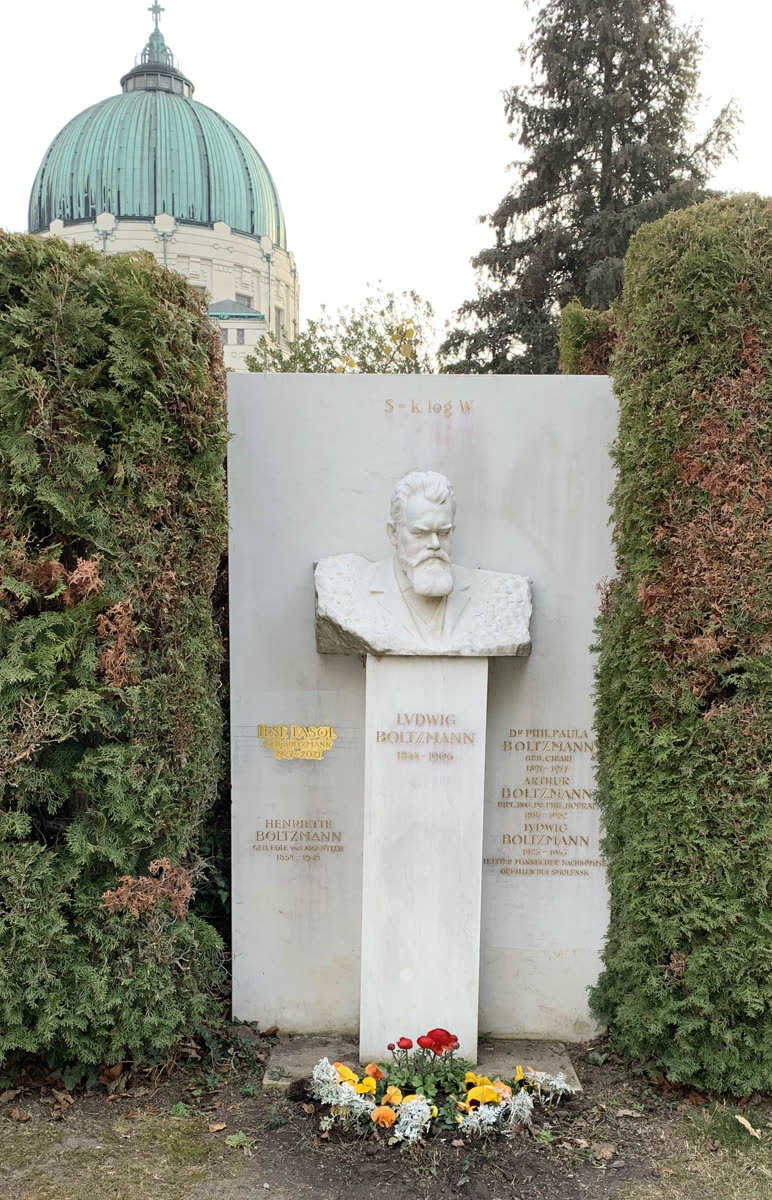
\includegraphics[width=\linewidth]{images/book4/boltzmann-grave.jpg}\par
{\footnotesize Het graf van Boltzmann.}
\end{minipage}
\end{history}

\section{Oefeningen}

\begin{exercise}[$\star$]\label{exo:b3:partition-functions:1}
Vier oscillatoren delen vier kwanta. Geef de verdelingen en het gewicht
van elke verdeling, en controleer dat ze optellen tot het aantal manieren
om vier ononderscheidbare kwanta over vier oscillatoren te plaatsen, $\binom{7}{3}$. Welke
verdelingen zijn de waarschijnlijkste?
\end{exercise}

\begin{exercise}[$\star$]\label{exo:b3:partition-functions:2}
Twee niet-ontaarde niveaus liggen \qty{2.5}{kJ/mol} uit elkaar. Bereken de
verhouding van hun \omterm{def:b3:partition-functions:boltzmann}{bezettingen} bij \qty{298.15}{K} en bij \qty{1000}{K}. Wat
is de limiet bij zeer hoge temperatuur?
\end{exercise}

\begin{exercise}[$\star$]\label{exo:b3:partition-functions:3}
% ledger: aw:Ar
Bereken de \omterm{def:b3:partition-functions:thermal-wavelength}{thermische golflengte} van een argonatoom bij \qty{298.15}{K} en
zijn translatietoestandssom in een volume van \qty{1}{dm^3}.
\end{exercise}

\begin{exercise}[$\star$]\label{exo:b3:partition-functions:4}
% ledger: diat:N2.Be, diat:N2.ae, diat:HCl.Be, diat:HCl.ae
Bereken met $B_0 = \qty{1.990}{cm^{-1}}$ (\ce{N2}) en \qty{10.440}{cm^{-1}} (\ce{H^{35}Cl}) voor elk
molecuul $\theta_{\mathrm R}$ en de rotatietoestandssom bij hoge
temperatuur, bij
\qty{298.15}{K}.
\end{exercise}

\begin{exercise}[$\star\star$]\label{exo:b3:partition-functions:5}
% ledger: diat:I2.we, diat:I2.wexe, diat:N2.we, diat:N2.wexe
De fundamentele golfgetallen van \ce{I2} en \ce{N2} zijn \qty{213.27}{cm^{-1}} en
\qty{2329.92}{cm^{-1}}. Bereken $\theta_{\mathrm V}$, $q^{\mathrm V}$ bij \qty{298.15}{K}, en de fractie
moleculen die zich niet in $v = 0$ bevinden.
\end{exercise}

\begin{exercise}[$\star\star$]\label{exo:b3:partition-functions:6}
% ledger: diat:NO.split, lev:Cl.2P1_2
Bereken bij \qty{298.15}{K} de elektronische toestandssom van \ce{NO} (twee
tweevoudig \omterm{def:b3:quantum-model-systems:degenerate}{ontaarde niveaus} die \qty{119.73}{cm^{-1}} uit elkaar liggen) en
van het chlooratoom (grondniveau ${}^2P_{3/2}$, ${}^2P_{1/2}$ bij \qty{882.35}{cm^{-1}}).
Welke fractie van de \ce{NO}-moleculen bevindt zich in het hogere niveau?
Waarnaar nadert $q^{\mathrm E}(\ce{NO})$ bij hoge temperatuur?
\end{exercise}

\begin{exercise}[$\star\star$]\label{exo:b3:partition-functions:7}
Leid uit $q^{\mathrm T} = V/\Lambda^3$ de inwendige energie en de
warmtecapaciteit bij constant volume af van één mol van een monoatomisch
ideaal gas, en bereken $U - U(0)$ bij
\qty{298.15}{K}.
\end{exercise}

\begin{exercise}[$\star\star$]\label{exo:b3:partition-functions:8}
% ledger: aw:Ar, s0:Ar_g
Bereken met de vergelijking van Sackur-Tetrode de standaard molaire
entropie van argon bij \qty{298.15}{K}; vergelijk met de getabelleerde
\qty{154.846}{J.K^{-1}.mol^{-1}}. Hoeveel verandert ze als de druk door 10
gedeeld wordt?
\end{exercise}

\begin{exercise}[$\star\star$]\label{exo:b3:partition-functions:9}
% ledger: diat:HCl.Be, diat:HCl.ae
Bereken de rotatiebijdrage tot de standaard molaire entropie van
\ce{H^{35}Cl} bij \qty{298.15}{K} ($\theta_{\mathrm R} = \qty{15.02}{K}$).
\end{exercise}

\begin{exercise}[$\star\star\star$]\label{exo:b3:partition-functions:10}
Toon aan, met $J$ behandeld als continu, dat het sterkst bezette
rotatieniveau van een lineair molecuul bij ongeveer $J_{\max} = \sqrt{T/2\theta_{\mathrm R}} - \frac12$
ligt. Bereken het voor \ce{HCl}
($\theta_{\mathrm R} = \qty{15.02}{K}$) en \ce{CO} ($\theta_{\mathrm R} = \qty{2.766}{K}$) bij \qty{300}{K}. Waarom zijn de twee
takken van een infraroodband het sterkst enkele lijnen van het midden?
\end{exercise}

\begin{exercise}[$\star\star\star$]\label{exo:b3:partition-functions:11}
% ledger: diat:H2.Be, diat:H2.ae
De formule van Euler-Maclaurin geeft $\sum_{J\ge0}f(J) \approx \int_0^\infty f(J)\dd J + \frac12f(0) -
\frac1{12}f'(0)$. Pas haar toe op $f(J) = (2J+1)\eu^{-\theta J(J+1)/T}$ en toon aan dat $q^{\mathrm R} \approx T/\theta +
\frac13$. Voor welke temperaturen is $T/\theta$ correct tot op 1\,\%? Is het
aanvaardbaar voor \ce{H2}
($B_0 = \qty{59.32}{cm^{-1}}$) bij \qty{298.15}{K}?
\end{exercise}

\begin{exercise}[$\star\star\star$]\label{exo:b3:partition-functions:12}
% ledger: diat:I2.we, diat:I2.wexe
Toon aan dat de molaire vibratie-entropie naar nul gaat wanneer $T \ll \theta_{\mathrm V}$ en naar
$R[1 + \ln(T/\theta_{\mathrm V})]$ wanneer $T \gg \theta_{\mathrm V}$. Bereken zowel de
exacte uitdrukking als deze limiet voor \ce{I2} ($\theta_{\mathrm V} = \qty{306.9}{K}$) bij \qty{298.15}{K}, en becommentarieer.
\end{exercise}

\section{Probleem: de entropie van stikstof tellen}

\begin{problem}[{Weekendprobleem --- de entropie van stikstof tellen: de
translatie-, rotatie-, vibratie- en elektronische bijdragen tot zijn
standaardentropie, berekend uit zijn spectrum en vergeleken met de tabel}]
\label{pb:b3:partition-functions:1}
% ledger: aw:N, diat:N2.Be, diat:N2.ae, diat:N2.we, diat:N2.wexe, s0:N2_g, const:h, const:kB, const:NA, const:c
Stikstof is het belangrijkste gas van de lucht. Zijn standaard molaire
entropie bij
\qty{298.15}{K} wordt hier berekend uit zijn molaire massa,
\qty{28.014}{g/mol}, en uit zijn spectroscopische constanten: $B_e = \qty{1.998241}{cm^{-1}}$, $\alpha_e = \qty{0.017318}{cm^{-1}}$, $\omega_e =
\qty{2358.57}{cm^{-1}}$, $\omega_ex_e = \qty{14.324}{cm^{-1}}$; zijn
elektronische grondterm is ${}^1\Sigma_g^+$.
Standaarddruk $p^\circ = \qty{1}{bar}$; $k = \qty{1.380649e-23}{J/K}$, $h = \qty{6.62607015e-34}{J.s}$.

\medskip\noindent\textbf{Deel I --- Translatie.}
\begin{enumerate}
  \item Bereken de massa van één molecuul.
  \item Bereken zijn \omterm{def:b3:partition-functions:thermal-wavelength}{thermische golflengte} bij \qty{298.15}{K}.
  \item Bereken het beschikbare volume per molecuul, $kT/p^\circ$.
  \item Leid $q^{\mathrm T}/N$ af, en becommentarieer de grootte ervan.
  \item Bereken de molaire translatie-entropie.
  \item Hoeveel zou ze veranderen bij de halve druk?
\end{enumerate}

\medskip\noindent\textbf{Deel II --- Rotatie.}
\begin{enumerate}[resume]
  \item Bereken $B_0$.
  \item Bereken $\theta_{\mathrm R}$.
  \item Geef het \omterm{def:b3:partition-functions:symmetry-number}{symmetriegetal} en zeg waarmee het rekening houdt.
  \item Bereken $q^{\mathrm R}$ bij \qty{298.15}{K}.
  \item Is de hogetemperatuurvorm gerechtvaardigd?
  \item Bereken de molaire rotatie-entropie.
  \item Welk rotatieniveau is het sterkst bezet, als je de gewichten van de
        kernspin verwaarloost?
\end{enumerate}

\medskip\noindent\textbf{Deel III --- Vibratie en elektronische toestanden.}
\begin{enumerate}[resume]
  \item Bereken het vibratiekwantum $G(1) - G(0)$.
  \item Bereken $\theta_{\mathrm V}$.
  \item Bereken $q^{\mathrm V}$ bij \qty{298.15}{K}.
  \item Welke fractie van de moleculen bevindt zich in $v = 1$?
  \item Bereken de molaire vibratie-entropie.
  \item Wat is de elektronische bijdrage? Waarom mogen aangeslagen
        elektronische toestanden verwaarloosd worden?
\end{enumerate}

\medskip\noindent\textbf{Deel IV --- Som en vergelijking.}
\begin{enumerate}[resume]
  \item Tel de bijdragen op.
  \item Vergelijk met de getabelleerde \qty{191.609}{J.K^{-1}.mol^{-1}}.
  \item Op welke metingen berust de calorimetrische waarde van een tabel?
  \item Waarom mogen de tabellen de kernspin weglaten?
  \item Formuleer het resultaat: de standaard molaire entropie van stikstof
        bij \qty{298.15}{K}, berekend uit zijn spectroscopische constanten.
\end{enumerate}
\end{problem}
